\pagebreak
\begin{center}
    \underline{\large \textbf{Pembahasan Latihan Soal Bab 1 dan Bab 2}}
\end{center}
\begin{tabular}{l l}
    Mata Kuliah & : Fisika 2 \\
    Kelas & : 44 \\
    Dosen & : Sefi Novendra Patrialova, S.Si., M.T. \\
    Asisten & : Surya Anoraga Justitia Yusman
\end{tabular}
\vskip10pt
\hrule
\vskip10pt
\noindent\underline{\textbf{Gaya Coulomb}}
\begin{enumerate}
    \item \underline{\textbf{Osilasi Muatan Akibat Muatan Lain}}
    \vskip5pt
    Dua muatan positif $+Q$ ditempatkan pada jarak $b$. Suatu muatan positif $+q$ dan massa $m$ diletakkan di antara kedua muatan ini. Kemudian muatan ini digerakkan sedikit searah dengan garis penghubung kedua muatan, lalu dilepaskan sehingga muatan akan berosilasi. Hitung periode osilasi ini! Hitung juga periode osilasi jika $+q$ diganti dengan $-q$ tetapi digerakkan dalam arah tegak lurus garis penghubung kedua muatan!
    
    a) $+q$ sejajar garis penghubung keuda muatan
    \begin{center}
        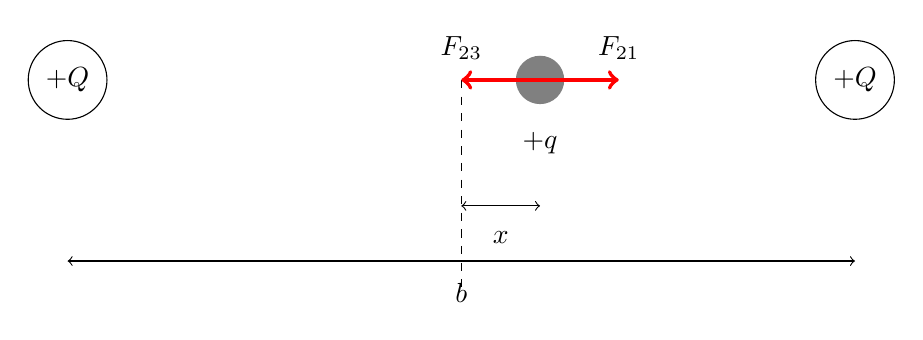
\begin{tikzpicture}
            \draw (-2,0) circle [radius=5mm];
            \filldraw[gray] (4,0) circle [radius=3mm]; 
            \draw (8,0) circle [radius=5mm];
            \node at (-2,0){$+Q$};
            \node at (8,0){$+Q$};
            \node at (4,-0.8){$+q$};
            %\node at (-2,0.8){$q_1$};
            %\node at (4,0.8){$q_2$};
            %\node at (8,0.8){$q_3$};
            \draw [<->] (-2,-2.3)--(8,-2.3);
            \draw [<->] (3,-1.6)--(4,-1.6);
            \node at (3.5,-2){$x$};
            \node at (3,-2.7){$b$};
            \draw[dashed] (3,0)--(3,-2.7);
            \filldraw [line width=1.5pt, red, <-] (3,0)--(4,0);
            \filldraw [line width=1.5pt, red, ->] (4,0)--(5,0);
            \node at (3,0.4){$F_{23}$};
            \node at (5,0.4){$F_{21}$};
        \end{tikzpicture}
    \end{center}

    \begin{minipage}{0.5\textwidth}
    \begin{align*}
    \sum F = ma\\
    -F_{23}+F_{21} = ma\\
    -\frac{kqQ}{(\frac{b}{2}-x)^{2}}+\frac{kqQ}{(\frac{b}{2}+x)^{2}} = ma\\
    -kqQ\left ( \frac{1}{(\frac{b}{2}-x)^{2}}-\frac{1}{(\frac{b}{2}+x)^{2}} \right) = ma\\
    -kqQ\left ( \frac{\left ( \frac{b}{2}+x \right)^{2}-\left ( \frac{b}{2}-x \right )^{2}}{\left ( \frac{b}{2}+x \right)^{2}\left ( \frac{b}{2}-x \right )^{2}} \right ) = ma\\
    -kqQ\left ( \frac{2b}{\left ( \left ( \frac{b}{2} \right )^{2} -x^{2}\right )^{2}} \right )x = ma
    \end{align*}
    Untuk $x$ sangat kecil maka $x^{2} \approx 0$, sehingga
    \end{minipage}
    \hfill
    \begin{minipage}{0.5\textwidth}
    \begin{align*}
    -kqQ\left ( \frac{2b}{\left ( \frac{b}{2} \right )^{4}} \right )x &=ma\\   
    -kqQ\left ( \frac{32}{b^{3}} \right )x &=m\frac{d^{2}x}{dt^{2}}\\ 
    \frac{d^{2}x}{dt^{2}} + \frac{32kqQ}{mb^{3}}x&=0\\
    \omega^{2}=\frac{32kqQ}{mb^{3}} \\
    \omega = \sqrt{\frac{32kqQ}{mb^{3}}} \\
    \frac{2\pi}{T}= \sqrt{\frac{32kqQ}{mb^{3}}} \\
    \fbox{$T = 2\pi\sqrt{\frac{mb^{3}}{32kqQ}}$}
    \end{align*}
    \end{minipage}
    
    \pagebreak
    b) $-q$ tegak lurus garis penghubung keuda muatan

    \begin{center}
        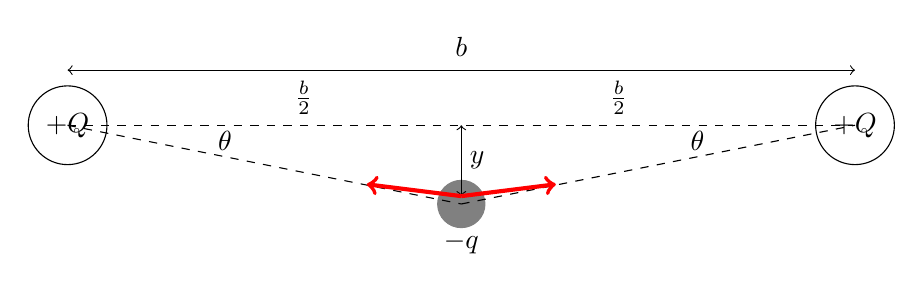
\begin{tikzpicture}
            \draw (-2,0) circle [radius=5mm];
            \filldraw[gray] (3,-1) circle [radius=3mm]; 
            \draw (8,0) circle [radius=5mm];
            \node at (-2,0){$+Q$};
            \node at (8,0){$+Q$};
            \node at (3,-1.5){$-q$};
            %\node at (-2,0.8){$q_1$};
            %\node at (4,0.8){$q_2$};
            %\node at (8,0.8){$q_3$};
            \draw [<->] (-2,0.7)--(8,0.7);
            \draw [<->] (3,0)--(3,-0.9);
            \node at (3.2,-0.45){$y$};
            \node at (3,1){$b$};
            \draw[dashed] (-2,0)--(3,-1);
            \draw[dashed] (3,-1)--(8,0);
            \draw[dashed](-2,0)--(8,0);
            \node at (1,0.35) {$\frac{b}{2}$};
            \node at (5,0.35) {$\frac{b}{2}$};
            \node at (0,-0.2) {$\theta$};
            \node at (6,-0.2) {$\theta$};
            \draw[red,line width=1.5pt,->](3,-0.9)--(1.8,-0.75);
            \draw[red,line width=1.5pt,->](3,-0.9)--(4.2,-0.75);
        \end{tikzpicture}
    \end{center}
    \begin{minipage}{0.5\textwidth}
    Gaya-gaya yang dialami muatan $-q$ pada \\ arah vertikal
    \begin{center}
        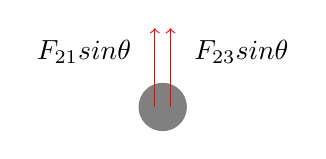
\begin{tikzpicture}
            \filldraw[gray] (0,0) circle [radius=3mm];
            \draw [red,->](-0.1,0)--(-0.1,1);
            \draw [red,->](0.1,0)--(0.1,1);
            \node at (-1,0.7){$F_{21}sin\theta$};
            \node at (1,0.7){$F_{23}sin\theta$};
        \end{tikzpicture}
    \end{center}
    \begin{align*}
    \sum F=ma\\
    -F_{21}sin\theta-F_{23}sin\theta=ma\\
    -\frac{kqQ}{\left ( \frac{b}{2}cos\theta \right )^{2}}sin\theta-\frac{kqQ}{\left ( \frac{b}{2}cos\theta \right )^{2}}sin\theta=ma\\
    -\frac{2kqQ}{\left ( \frac{b}{2}cos\theta \right )^{2}}sin\theta=ma \\    
    \end{align*}
    
    \end{minipage}
    \hfill
    \begin{minipage}{0.4\textwidth}
    Untuk sudut kecil $cos\theta \approx 1$ \\ dan $sin\theta \approx \theta$
    \begin{align*}
    -\frac{2kqQ}{\left ( \frac{b}{2} \right )^{2}}\theta=ma \\
    -\frac{8kqQ}{b^{2}}\theta=ma \\
    -\frac{8kqQ}{b^{2}}\frac{y}{\frac{b}{2}}=m\frac{d^{2}y}{dt^{2}} \\
    \frac{d^{2}y}{dt^{2}}+\frac{16kqQ}{mb^{3}}y=0 \\
    \omega^{2}=\frac{16kqQ}{mb^{3}}\\
    \frac{2\pi}{T}=\sqrt{\frac{16kqQ}{mb^{3}}}\\
    \fbox{$T=2\pi\sqrt{\frac{mb^{3}}{16kqQ}}$}
    \end{align*}
    \end{minipage}
\end{enumerate}
